%%%%%%%%%%%%%%%%%%%%%%%%%%%%%%%%%%%%%%%%%
% Programming/Coding Assignment
% LaTeX Template
%
% This template has been downloaded from:
% http://www.latextemplates.com
%
% Original author:
% Ted Pavlic (http://www.tedpavlic.com)
%
% Note:
% The \lipsum[#] commands throughout this template generate dummy text
% to fill the template out. These commands should all be removed when 
% writing assignment content.
%
% This template uses a Perl script as an example snippet of code, most other
% languages are also usable. Configure them in the "CODE INCLUSION 
% CONFIGURATION" section.
%
%%%%%%%%%%%%%%%%%%%%%%%%%%%%%%%%%%%%%%%%%

%----------------------------------------------------------------------------------------
% PACKAGES AND OTHER DOCUMENT CONFIGURATIONS
%----------------------------------------------------------------------------------------

\documentclass{article}

\usepackage{fancyhdr} % Required for custom headers
\usepackage{lastpage} % Required to determine the last page for the footer
\usepackage{extramarks} % Required for headers and footers
\usepackage[usenames,dvipsnames]{color} % Required for custom colors
\usepackage{graphicx} % Required to insert images
\usepackage{listings} % Required for insertion of code
\usepackage{courier} % Required for the courier font
\usepackage{lipsum} % Used for inserting dummy 'Lorem ipsum' text into the template
\usepackage{hyperref}

% Margins
\topmargin=-0.45in
\evensidemargin=0in
\oddsidemargin=0in
\textwidth=6.5in
\textheight=9.0in
\headsep=0.25in

\linespread{1.1} % Line spacing

% Set up the header and footer
\pagestyle{fancy}
\lhead{\hmwkAuthorName} % Top left header
% \chead{\firstxmark} % Top right header
\rhead{\hmwkClass\ (\hmwkClassInstructor\ \hmwkClassTime): \hmwkTitle} % Top center head
\lfoot{} % Bottom left footer
\cfoot{} % Bottom center footer
\rfoot{Page\ \thepage\ of\ \protect\pageref{LastPage}} % Bottom right footer
\renewcommand\headrulewidth{0.4pt} % Size of the header rule
\renewcommand\footrulewidth{0.4pt} % Size of the footer rule

\setlength\parindent{0pt} % Removes all indentation from paragraphs

%----------------------------------------------------------------------------------------
% CODE INCLUSION CONFIGURATION
%----------------------------------------------------------------------------------------

\definecolor{MyDarkGreen}{rgb}{0.0,0.4,0.0} % This is the color used for comments
\lstloadlanguages{Perl} % Load Perl syntax for listings, for a list of other languages supported see: ftp://ftp.tex.ac.uk/tex-archive/macros/latex/contrib/listings/listings.pdf
\lstset{language=Perl, % Use Perl in this example
        frame=single, % Single frame around code
        basicstyle=\small\ttfamily, % Use small true type font
        keywordstyle=[1]\color{Blue}\bf, % Perl functions bold and blue
        keywordstyle=[2]\color{Purple}, % Perl function arguments purple
        keywordstyle=[3]\color{Blue}\underbar, % Custom functions underlined and blue
        identifierstyle=, % Nothing special about identifiers                                         
        commentstyle=\usefont{T1}{pcr}{m}{sl}\color{MyDarkGreen}\small, % Comments small dark green courier font
        stringstyle=\color{Purple}, % Strings are purple
        showstringspaces=false, % Don't put marks in string spaces
        tabsize=5, % 5 spaces per tab
        %
        % Put standard Perl functions not included in the default language here
        morekeywords={rand},
        %
        % Put Perl function parameters here
        morekeywords=[2]{on, off, interp},
        %
        % Put user defined functions here
        morekeywords=[3]{test},
        %
        morecomment=[l][\color{Blue}]{...}, % Line continuation (...) like blue comment
        numbers=left, % Line numbers on left
        firstnumber=1, % Line numbers start with line 1
        numberstyle=\tiny\color{Blue}, % Line numbers are blue and small
        stepnumber=5 % Line numbers go in steps of 5
}

% Creates a new command to include a perl script, the first parameter is the filename of the script (without .pl), the second parameter is the caption
\newcommand{\perlscript}[2]{
\begin{itemize}
\item[]\lstinputlisting[caption=#2,label=#1]{#1.pl}
\end{itemize}
}

%----------------------------------------------------------------------------------------
% DOCUMENT STRUCTURE COMMANDS
% Skip this unless you know what you're doing
%----------------------------------------------------------------------------------------

% Header and footer for when a page split occurs within a problem environment
\newcommand{\enterProblemHeader}[1]{
\nobreak\extramarks{#1}{#1 continued on next page\ldots}\nobreak
\nobreak\extramarks{#1 (continued)}{#1 continued on next page\ldots}\nobreak
}

% Header and footer for when a page split occurs between problem environments
\newcommand{\exitProblemHeader}[1]{
\nobreak\extramarks{#1 (continued)}{#1 continued on next page\ldots}\nobreak
\nobreak\extramarks{#1}{}\nobreak
}

\setcounter{secnumdepth}{0} % Removes default section numbers
\newcounter{homeworkProblemCounter} % Creates a counter to keep track of the number of problems

\newcommand{\homeworkProblemName}{}
\newenvironment{homeworkProblem}[1][Question \arabic{homeworkProblemCounter}]{ % Makes a new environment called homeworkProblem which takes 1 argument (custom name) but the default is "Problem #"
\stepcounter{homeworkProblemCounter} % Increase counter for number of problems
\renewcommand{\homeworkProblemName}{#1} % Assign \homeworkProblemName the name of the problem
\section{\homeworkProblemName} % Make a section in the document with the custom problem count
\enterProblemHeader{\homeworkProblemName} % Header and footer within the environment
}{
\exitProblemHeader{\homeworkProblemName} % Header and footer after the environment
}

\newcommand{\problemAnswer}[1]{ % Defines the problem answer command with the content as the only argument
\noindent\framebox[\columnwidth][c]{\begin{minipage}{0.98\columnwidth}#1\end{minipage}} % Makes the box around the problem answer and puts the content inside
}

\newcommand{\homeworkSectionName}{}
\newenvironment{homeworkSection}[1]{ % New environment for sections within homework problems, takes 1 argument - the name of the section
\renewcommand{\homeworkSectionName}{#1} % Assign \homeworkSectionName to the name of the section from the environment argument
\subsection{\homeworkSectionName} % Make a subsection with the custom name of the subsection
\enterProblemHeader{\homeworkProblemName\ [\homeworkSectionName]} % Header and footer within the environment
}{
\enterProblemHeader{\homeworkProblemName} % Header and footer after the environment
}

%----------------------------------------------------------------------------------------
% NAME AND CLASS SECTION
%----------------------------------------------------------------------------------------

\newcommand{\hmwkTitle}{Assignment\ \#4} % Assignment title
\newcommand{\hmwkDueDate}{Friday,\ April\ 30,\ 2015} % Due date
\newcommand{\hmwkClass}{Introduction to Digital Libraries\ CS-751} % Course/class
\newcommand{\hmwkClassTime}{4:20pm} % Class/lecture time
\newcommand{\hmwkClassInstructor}{Michael L. Nelson} % Teacher/lecturer
\newcommand{\hmwkAuthorName}{Avinash Gosavi} % Your name

%----------------------------------------------------------------------------------------
% TITLE PAGE
%----------------------------------------------------------------------------------------

\title{
\vspace{2in}
\textmd{\textbf{\hmwkClass}}\\
\textmd{\textbf{\hmwkTitle}}\\
\normalsize\vspace{0.1in}\small{Due\ on\ \hmwkDueDate}\\
\vspace{0.1in}\large{\textit{\hmwkClassInstructor\ \hmwkClassTime}}
\vspace{3in}
}

\author{\textbf{\hmwkAuthorName}}
\date{} % Insert date here if you want it to appear below your name

%----------------------------------------------------------------------------------------


\bibliographystyle{plain}
\bibliography{reference}

\begin{document}

\maketitle

%----------------------------------------------------------------------------------------
% TABLE OF CONTENTS
%----------------------------------------------------------------------------------------

%\setcounter{tocdepth}{1} % Uncomment this line if you don't want subsections listed in the ToC

\newpage
\tableofcontents
\newpage

%----------------------------------------------------------------------------------------
% PROBLEM 1
%----------------------------------------------------------------------------------------

% To have just one problem per page, simply put a \clearpage after each problem

\begin{homeworkProblem}
Using the pages from A3 that boilerpipe successfully processed, download those representations again \& reprocess them with boilerpipe.  

\begin{itemize}

  \item Document the time difference (e.g., Time(A4) – Time(A3)).
  \item Compute the Jaccard Distance x for each pair of pages (i.e., P(A3) \& P(A4) for:
  \begin{itemize}
    \item Unique terms (i.e., unigrams)
    \item Bigrams
    \item Trigrams
  \end{itemize}
  \item See: 
    \url{http://en.wikipedia.org/wiki/Jaccard_index}
  \item For each of the 3 cases (i.e., 1-, 2-, 3-grams) build a Cumulative Distribution Function that shows the \% change on the x-axis \& the \% of the population on the x-axis
  \item See: 
    \url{http://en.wikipedia.org/wiki/Cumulative_distribution_function}
  \item Give 3-4 examples illustrating the range of change that you have measured. \ldots

\end{itemize}

\end{homeworkProblem}

\section{Answer}

The boilerpipe files for A3 were extracted on Apr 1rd and for A4 were extracted on May 1. So, Around 30 days difference.\

% Some examples that I would like to mention are as below:-\
% \begin{itemize}
%     \item 
%     \item 
%     \item 
%   \end{itemize}

\clearpage

\subsection{Code Listing}
\subsubsection{Ngrams}

\lstinputlisting[language=Ruby,breaklines = true,frame=single,caption={Ngram Class}, label=lst:q1-1,captionpos=b,numbers=left,showspaces=false,showstringspaces=false,basicstyle=\footnotesize]{ngrams.rb}

\subsubsection{Jaccard Index}

\lstinputlisting[language=Ruby,breaklines = true,frame=single,caption={Jaccard Class}, label=lst:q1-1,captionpos=b,numbers=left,showspaces=false,showstringspaces=false,basicstyle=\footnotesize]{jaccard_index.rb}
\newpage

\subsubsection{File Ngrams}

\lstinputlisting[language=Ruby,breaklines = true,frame=single,caption={Jaccard Class}, label=lst:q1-1,captionpos=b,numbers=left,showspaces=false,showstringspaces=false,basicstyle=\footnotesize]{file_ngrams.rb}

\subsubsection{Save Ngrams Graph}

\lstinputlisting[language=Ruby,breaklines = true,frame=single,caption={Jaccard Class}, label=lst:q1-1,captionpos=b,numbers=left,showspaces=false,showstringspaces=false,basicstyle=\footnotesize]{save_ngrams.rb}
\newpage

\clearpage

\section{Figures}

\begin{center}
\begin{figure}[ht]
    \centering
    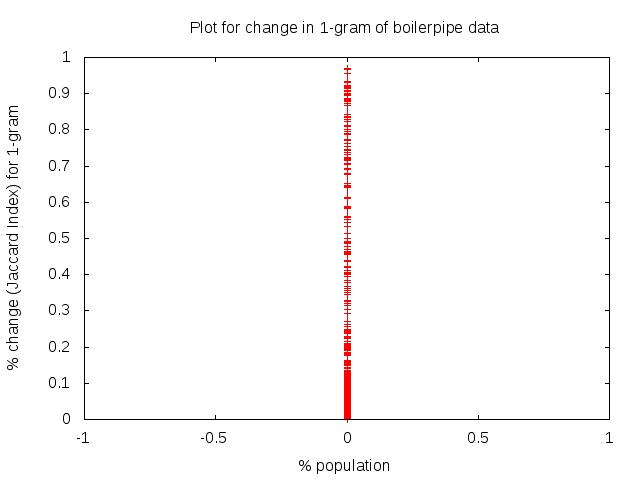
\includegraphics[width=0.475\textwidth,natwidth=700,natheight=700]{one_gram.png}
    \caption{Unigram}
    \label{fig:one_gram.png}
\end{figure}
\end{center}

\begin{center}
\begin{figure}[ht]
    \centering
    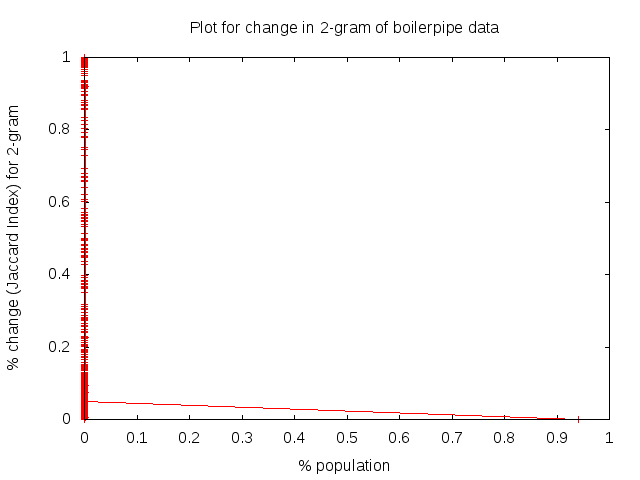
\includegraphics[width=0.475\textwidth,natwidth=700,natheight=700]{two_gram.png}
    \caption{Bigram}
    \label{fig:two_gram.png}
\end{figure}
\end{center}

\begin{center}
\begin{figure}[ht]
    \centering
    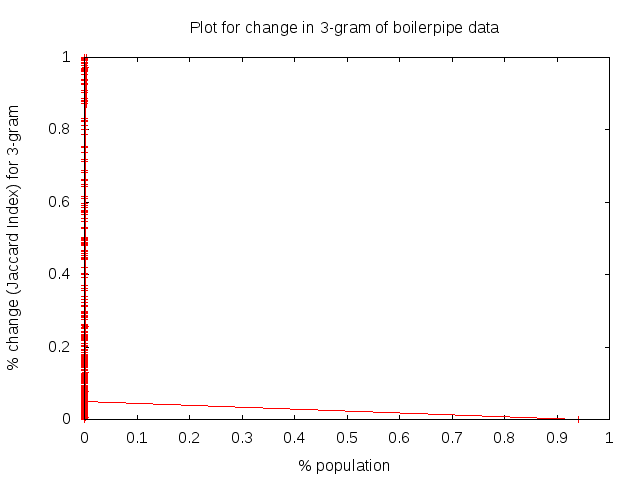
\includegraphics[width=0.475\textwidth,natwidth=700,natheight=700]{three_gram.png}
    \caption{Trigram}
    \label{fig:three_gram.png}
\end{figure}
\end{center}

\clearpage

%----------------------------------------------------------------------------------------
% PROBLEM 2
%----------------------------------------------------------------------------------------

\begin{homeworkProblem}

\begin{itemize}

  \item Using the pages from Q1 (A4), download all TimeMaps (including TimeMaps with 404 responses, i.e. empty or null TimeMaps)
  \begin{itemize}
    \item Upload all the TimeMaps to github
  \end{itemize}
  \item Build a CDF for \# of mementos for each original URI (i.e., x-axis = \# of mementos, y-axis = \% of links)
  \item See: 
    \url{http://timetravel.mementoweb.org/guide/api/}

\end{itemize}

\end{homeworkProblem}

\section{Answer}

Code used for finding no of Memento's are given below. From the graph built it can be observed that only a few URL's had more than 200 memento's. While quite few of them had 0 Memento's but, the reason for that may be that the pages were built recently.

\subsection{Code Listing}
\subsubsection{No of Mementos}

\lstinputlisting[language=Ruby,breaklines = true,frame=single,caption={Ngram Class}, label=lst:q1-1,captionpos=b,numbers=left,showspaces=false,showstringspaces=false,basicstyle=\footnotesize]{no_of_timemaps_graph.rb}

\newpage

\clearpage

\section{Figures}

\begin{center}
\begin{figure}[ht]
    \centering
    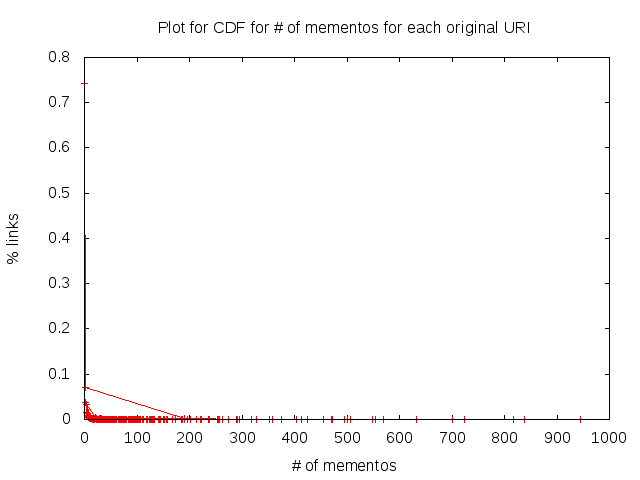
\includegraphics[width=0.475\textwidth,natwidth=700,natheight=700]{no_of_mementos.png}
    \caption{No of Mementos}
    \label{fig:no_of_mementos.png}
\end{figure}
\end{center}

\clearpage

%----------------------------------------------------------------------------------------
% PROBLEM 3
%----------------------------------------------------------------------------------------

\begin{homeworkProblem}

\begin{itemize}

  \item Using 20 links that have TimeMaps
  \begin{itemize}
    \item With >= 20 mementos
    \item Have existed >= 2 years (i.e., Memento-Datetime of \"first memento\" is April XX, 2013 or older)
    \item Note: select from Q1/Q2 links, else choose them by hand
  \end{itemize}
  \item Build a CDF for \# of mementos for each original URI (i.e., x-axis = \# of mementos, y-axis = \% of links)
  \begin{itemize}
    \item Upload all the TimeMaps to github
  \end{itemize}

\end{itemize}

\end{homeworkProblem}

\section{Answer}

Selected 20 URL's according to no of mementos found for the link. From the different CDF's we can observe various pattern for changes in links. I have listed a few of the CDF's below which looked interesting.

\subsection{Code Listing}
\subsubsection{Fetch Boiler for choosen 20}

\lstinputlisting[language=Ruby,breaklines = true,frame=single,caption={Ngram Class}, label=lst:q1-1,captionpos=b,numbers=left,showspaces=false,showstringspaces=false,basicstyle=\footnotesize]{get_boiler_pipe.rb}

\newpage

\subsubsection{Draw CDF for choosen 20}

\lstinputlisting[language=Ruby,breaklines = true,frame=single,caption={Ngram Class}, label=lst:q1-1,captionpos=b,numbers=left,showspaces=false,showstringspaces=false,basicstyle=\footnotesize]{get_jaccard_distance.rb}

\newpage

\section{Figures}

\begin{center}
\begin{figure}[ht]
    \centering
    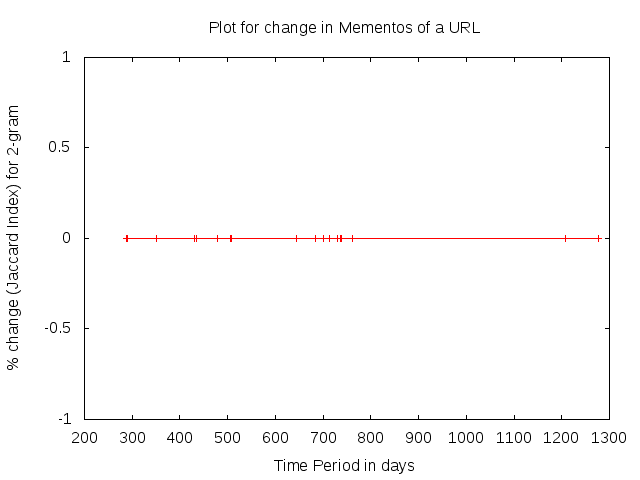
\includegraphics[width=0.475\textwidth,natwidth=700,natheight=700]{choosen_20_11.png}
    \caption{No change for a long time}
    \label{fig:choosen_20_11.png}
\end{figure}
\end{center}

\begin{center}
\begin{figure}[ht]
    \centering
    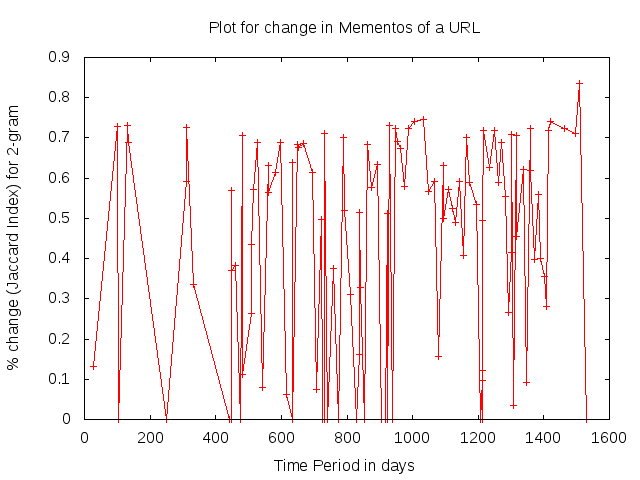
\includegraphics[width=0.475\textwidth,natwidth=700,natheight=700]{choosen_20_20.png}
    \caption{Frequently Changing Site}
    \label{fig:choosen_20_20.png}
\end{figure}
\end{center}

\begin{center}
\begin{figure}[ht]
    \centering
    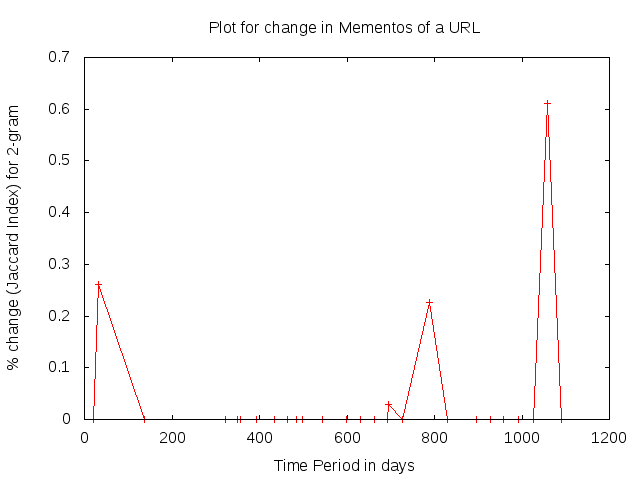
\includegraphics[width=0.475\textwidth,natwidth=700,natheight=700]{choosen_20_15.png}
    \caption{Rise and Fall in Changes}
    \label{fig:choosen_20_15.png}
\end{figure}
\end{center}

\clearpage

%----------------------------------------------------------------------------------------
% PROBLEM 4
%----------------------------------------------------------------------------------------

\begin{homeworkProblem}

\begin{itemize}

  \item Choose a news-related event
  \item Use twarc.py to collect 1000 tweets, every day for 5 different days
  
  \begin{itemize}
    \item See:
    \url{https://github.com/edsu/twarc}
  \end{itemize}
  
  \item For each day:
  \begin{itemize}
    \item Create a wall
    \item Build a tag/word cloud for each day
    \item Create a map using GeoJSON \& Github
    \begin{itemize}
        \item
        \url{https://help.github.com/articles/mapping-geojson-files-on-github/}
    \end{itemize}
  \end{itemize}
  \item Discuss in detail lessons learned, experiences, etc.

\end{itemize}

\end{homeworkProblem}

\section{Answer}

I have attached screenshot for wall, wordcloud and geojson for day of all the tweets I have collected.

The tool seems pretty cool and is really useful if you want to see what people are talking about from tag cloud, where people are talking from by using geojson and finally see all the actual tweets in wall type layout to read.

Didn't find anything difficult in generating all those files using the utilities provided in Twarc.

My key word was \"railsconf\" as there was a conference going on.

\section{Figures}

\begin{center}
\begin{figure}[ht]
    \centering
    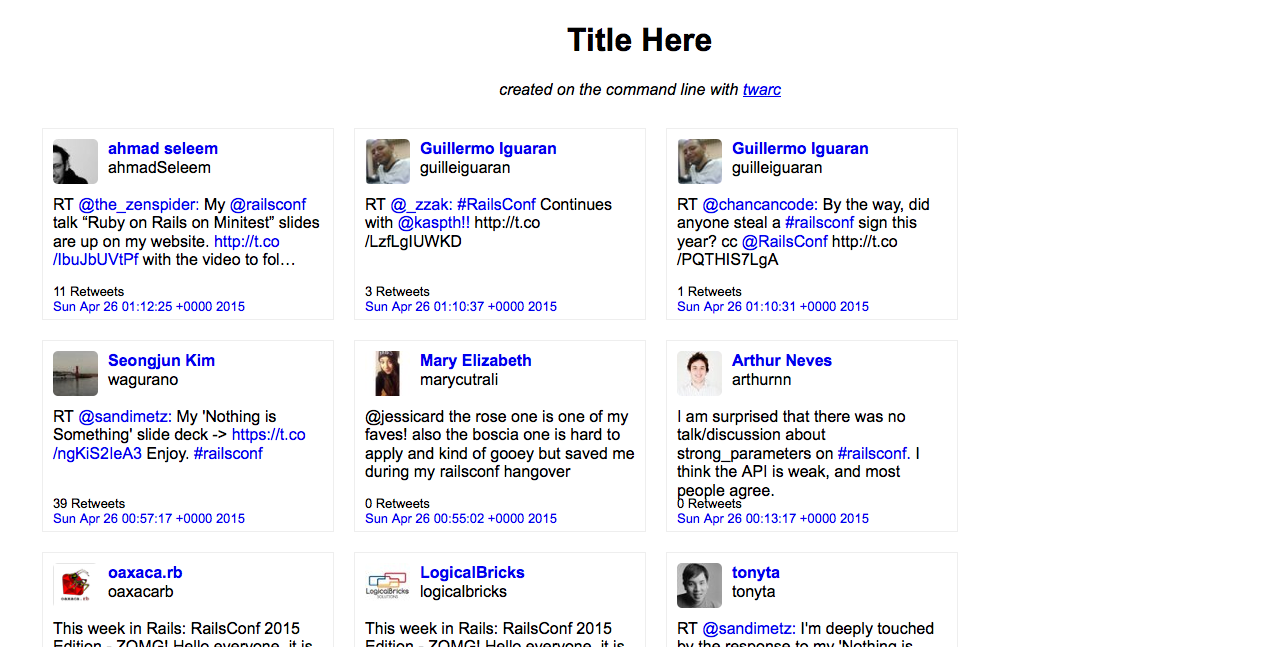
\includegraphics[width=0.475\textwidth,natwidth=700,natheight=700]{day 1 tweet wall.png}
    \caption{No of Mementos}
    \label{fig:day 1 tweet wall.png}
\end{figure}
\end{center}

\begin{center}
\begin{figure}[ht]
    \centering
    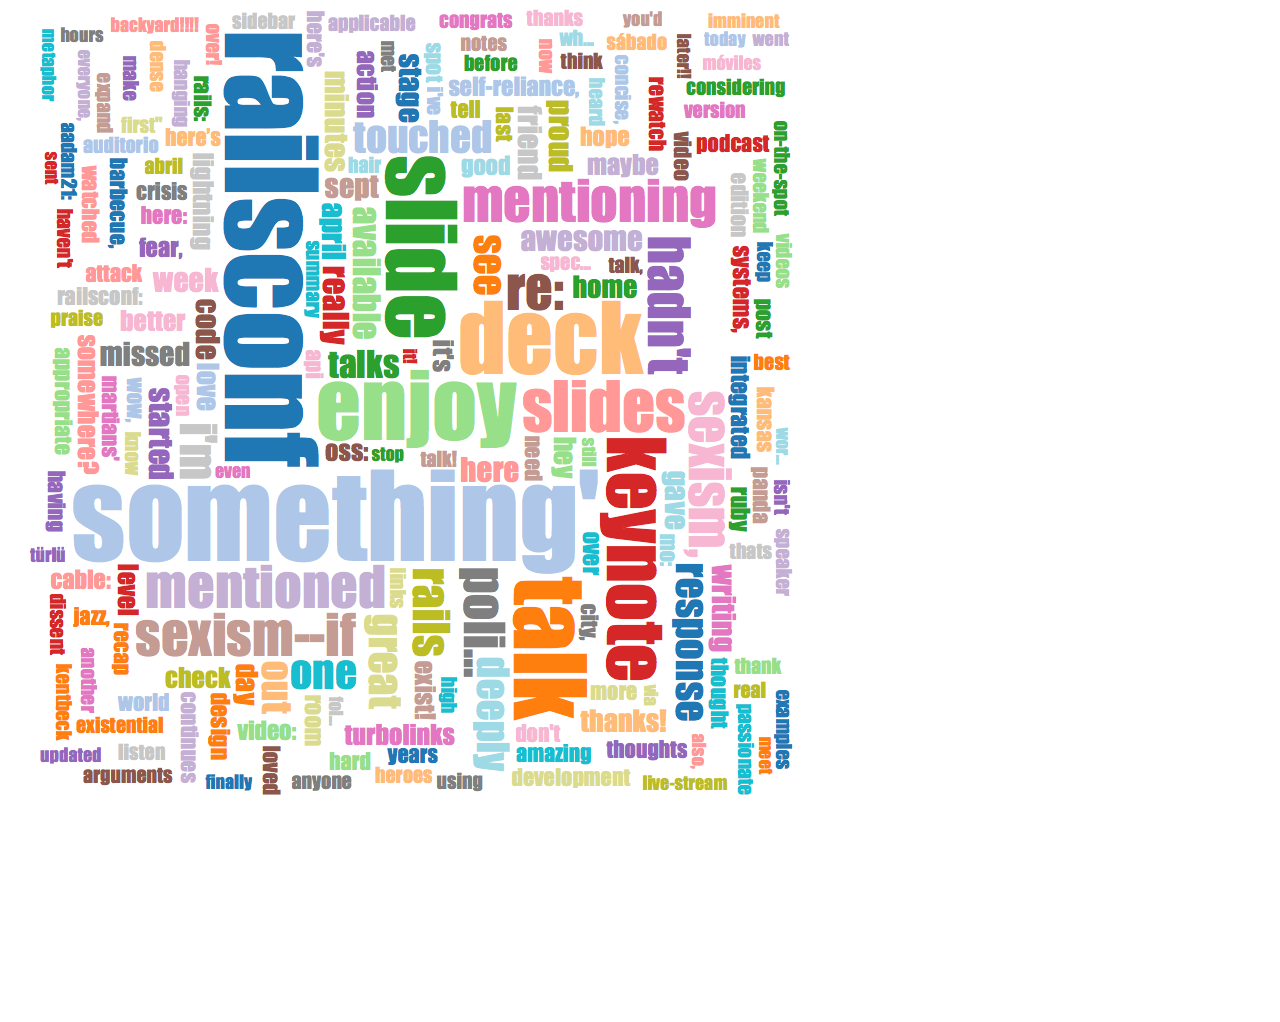
\includegraphics[width=0.475\textwidth,natwidth=700,natheight=700]{day 1 tweet wordcloud.png}
    \caption{No of Mementos}
    \label{fig:day 1 tweet wordcloud.png}
\end{figure}
\end{center}

\begin{center}
\begin{figure}[ht]
    \centering
    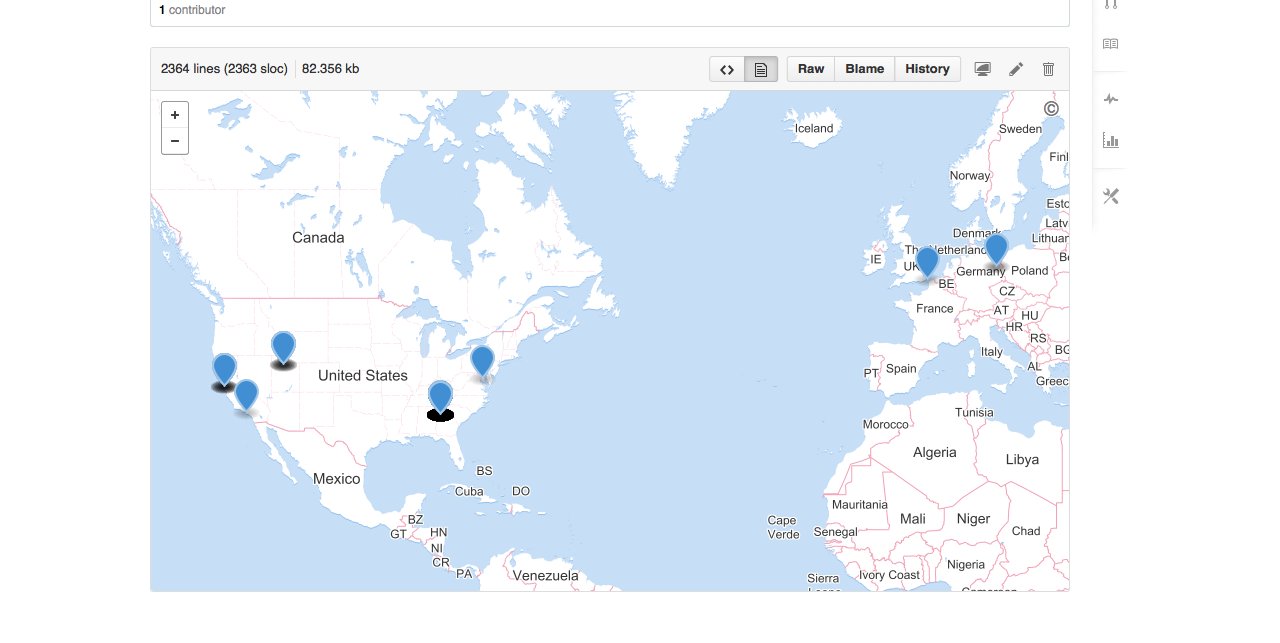
\includegraphics[width=0.475\textwidth,natwidth=700,natheight=700]{day 1 tweet geojson.png}
    \caption{No of Mementos}
    \label{fig:day 1 tweet geojson.png}
\end{figure}
\end{center}

\clearpage

\end{document}